\section{Análise de viabilidade técnica - simulação}

Nesta seção, será seguido o planejamento visto na metodologia~\ref{metodologia}.
Entretanto, vale antes destacar as variáveis do processo de revestimento,
utilizados durante toda a simulação:

\begin{itemize}
  \item A pistola de revestimento foi aproximada por um cilindro de 300 mm de
  comprimento e 50 mm de raio. Está acoplada à extremidade do efetuador,
  aumentando seu alcance em 300 mm.
  \item As pás da turbina podem girar em seu próprio eixo de $0^o$ a $29^o$.
  \item O rotor da turbina pode girar de $0^o$ a $360^o$.
  \item A distância entre extremidade da pistola e pá deve ser mantida em $235
  \pm 5$ mm durante toda a operação.
  \item O ângulo entre a pistola e o plano da pá deve ser $90^o \pm 60^o$, mas
  é aconselhável uma tolerância máxima de $30^o$.
\end{itemize}

\subsection{Modelo em CAD dos componentes da turbina}

Através da plataforma Solidworks, foram modelados elementos da turbina
necessários para a simulação. Após modelagem, os componentes são importados no
OpenRAVE no formato .wrl: aro câmara, rotor, íris, pá do rotor, e robô MH12 da
Motoman, objeto de estudo da simulação (figura~\ref{fig::arocamara}).

\begin{figure}[!ht]
	\centering	
	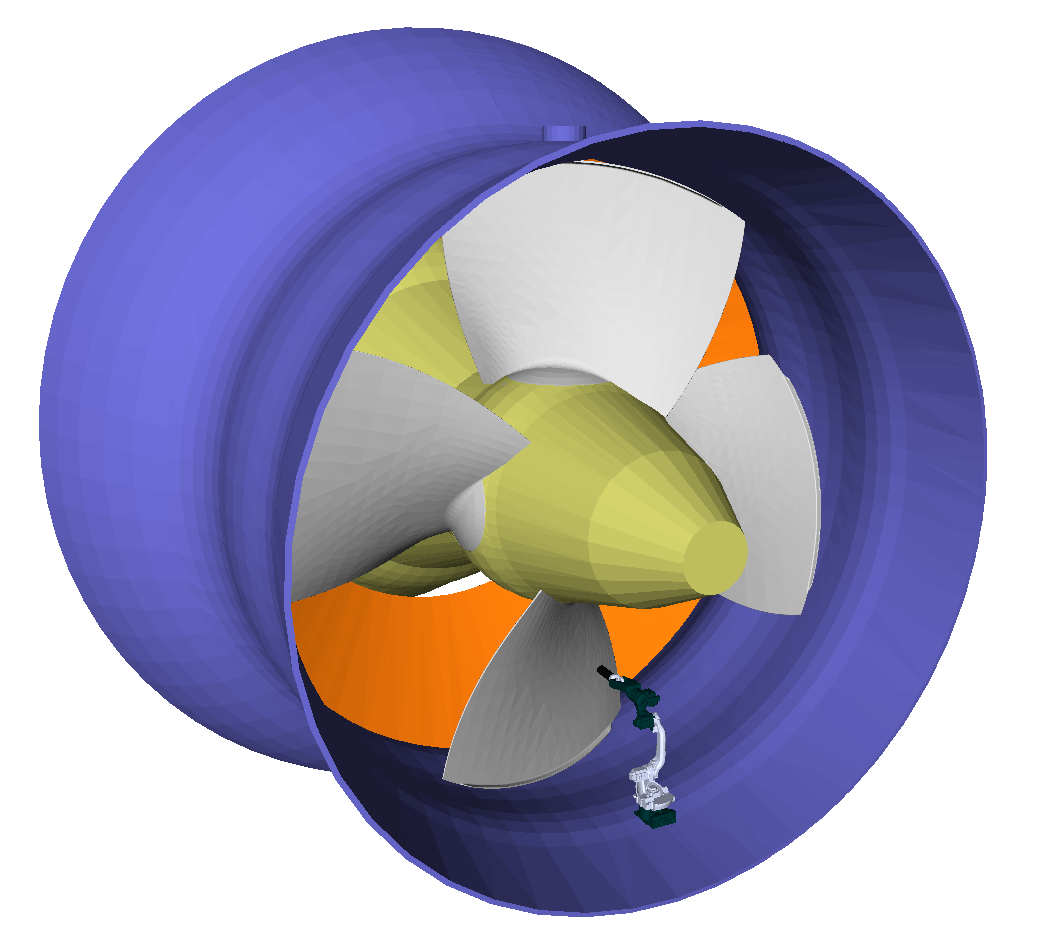
\includegraphics[width=.5\columnwidth]{figs/arocamara.png}
	\caption{Modelo CAD dos componentes da turbina e robô.}
	\label{fig::arocamara}
\end{figure}

\subsection{Discretização da pá}

A superfície da pá é amostrada, formando uma grade de tamanho fixo. A técnica
\textit{axis-aligned bounding box (AABB)} é utilizada para obter os
pontos e suas respectivas normais, na superfície da pá. Nesta técnica, a
superfície alvo é inscrita em um bloco, que é uniformemente amostrado. É, então,
realizada uma verificação de colisão entre os pontos amostrados no bloco e a
superfície alvo e, caso haja interseção, o ponto é armazenado junto com sua
normal à superfície. Dessa forma, podemos amostrar a pá e deslocar estes pontos
230 mm em relação à sua normal com a superfície, garantindo a requerimento do
revestimento. A representação dos pontos amostrados e deslocados em relação às
normais da pá estão nas figuras~\ref{fig::amostrapa1} e ~\ref{fig::amostrapa2}. 

\begin{figure}[!ht]
	\centering	
	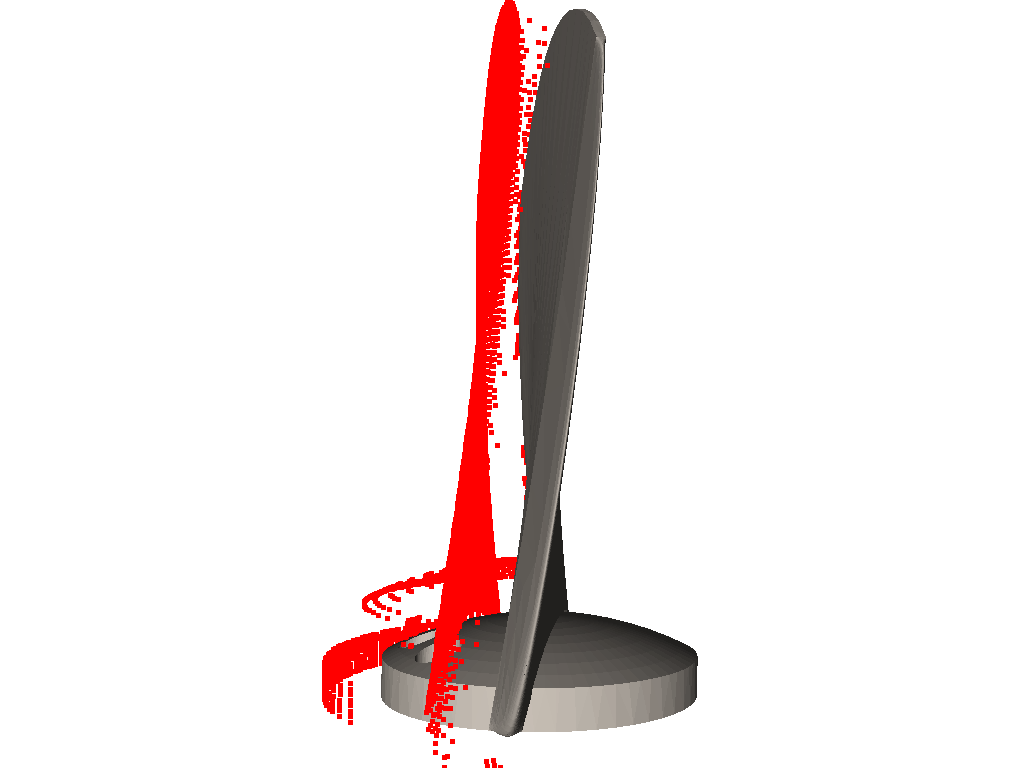
\includegraphics[width=.3\columnwidth]{figs/amostrapa1.png}
	\caption{Pontos amostrados da pá - vista lateral}
	\label{fig::amostrapa1}
\end{figure}

\begin{figure}[!ht]	
	\centering
	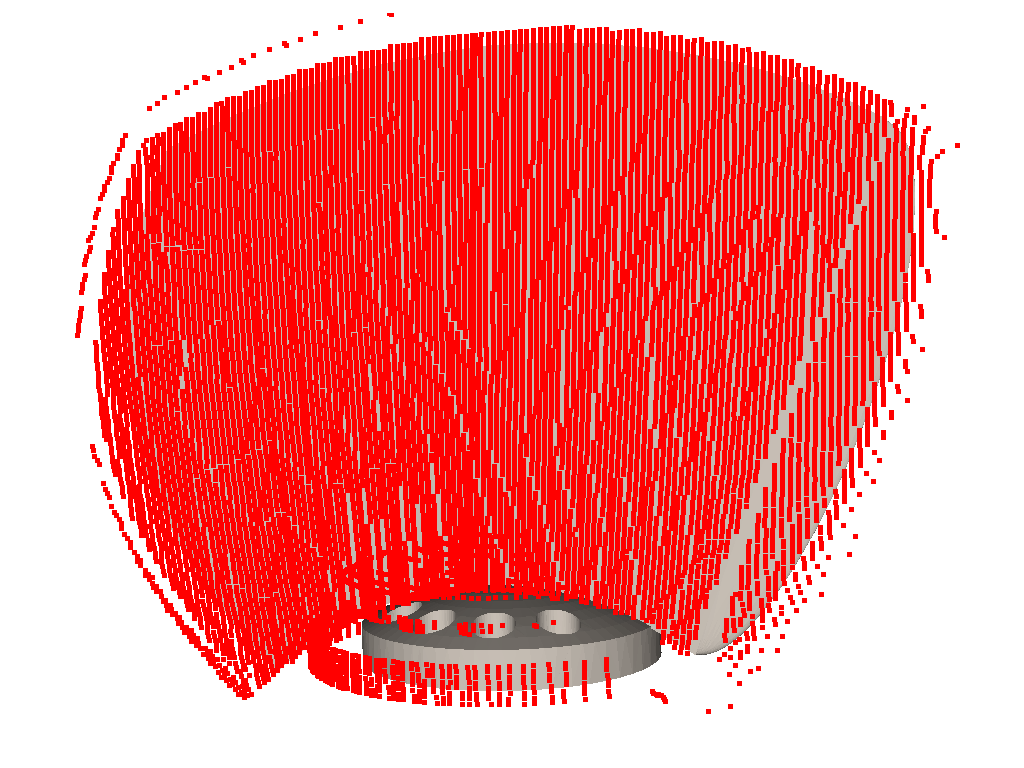
\includegraphics[width=.3\columnwidth]{figs/amostrapa2.png}
	\caption{Pontos amostrados da pá - vista frontal}
	\label{fig::amostrapa2}
\end{figure}

A técnica AABB realizada no OpenRAVE é semelhante ao
planejamento inicial para uma tarefa do tipo \textit{grasping}, na qual um robô
manipulador deve agarrar um objeto e, portanto, necessita reconhecer o seu
formato, e como se aproximar pelos vetores normais. Como a pá da turbina, alguns
objetos podem ser muito irregulares, de forma que amostras uniformes na
superfície do bloco não geram amostras uniformes na superfície do objeto
(figuras~\ref{fig::boundingbox} e ~\ref{fig::sampling}). A fim de garantir um
passo de amostragem próximo à resolução mínima do revestimento (3 mm), é
realizada uma superamostragem de 0.1 mm no bloco e aplica-se um filtro de 1 mm
na superfície da pá. O filtro busca por pontos na pá com distância inferior a 1
mm, mantendo um e deletando os vizinhos próximos. Em relação ao custo
computacional, o filtro foi implementado de maneira ótima pela técnica do
KDTree \cite{wald2006building}.

\begin{figure}[!ht]	
	\centering
	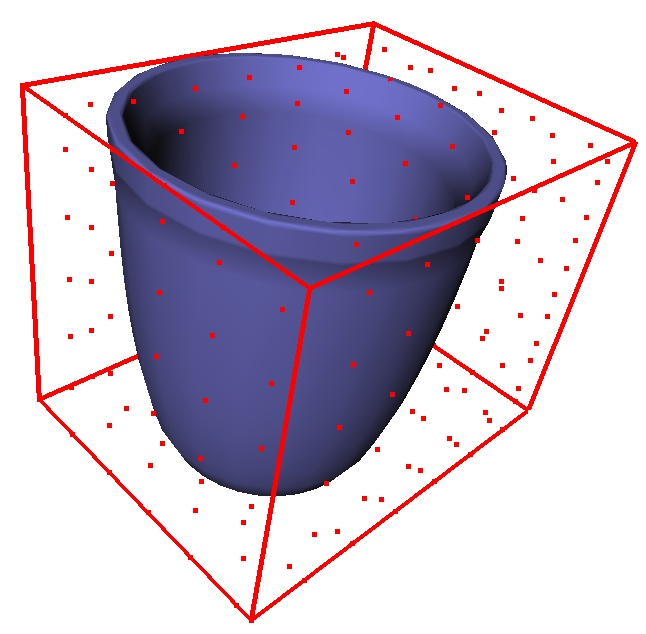
\includegraphics[width=.3\columnwidth]{figs/boundingbox.jpg}
	\caption{Amostras uniformes na superfície do bloco.}
	\label{fig::boundingbox}
\end{figure}

\begin{figure}[!ht]
	\centering	
	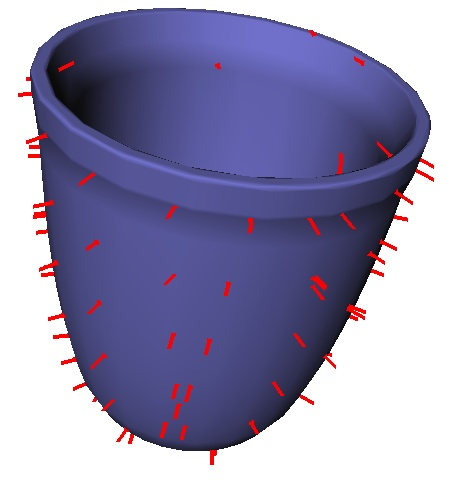
\includegraphics[width=.3\columnwidth]{figs/sampling.jpg}
	\caption{Amostras não uniformes na superfície do objeto.}
	\label{fig::sampling}
\end{figure}

\subsection{Simulação 1 - Extremidades da pá}

É fácil observar que as áreas de mais difícil acesso à pá são suas extremidades,
áreas em preto da figura~\ref{fig::extremidades}, devido ao alcance do robô e
por serem áreas em que a pá apresenta maior inclinação, o que afeta bastante na
direção dos vetores normais à pá. A alteração da direção da normal e a posição
do ponto a ser revestido são os fatores mais importantes para o aplicação de
revestimento, logo pontos em uma posição elevada para o robô e normal
direcionada para cima são complexos. Observe a figura~\ref{fig::normal}, o vetor
$\vec{P}$ é um exemplo de vetor normal pertencente a um ponto da pá de difícil
revestimento, tanto pela posição quanto pelo vetor normal.

\begin{figure}[!ht]
	\centering	
	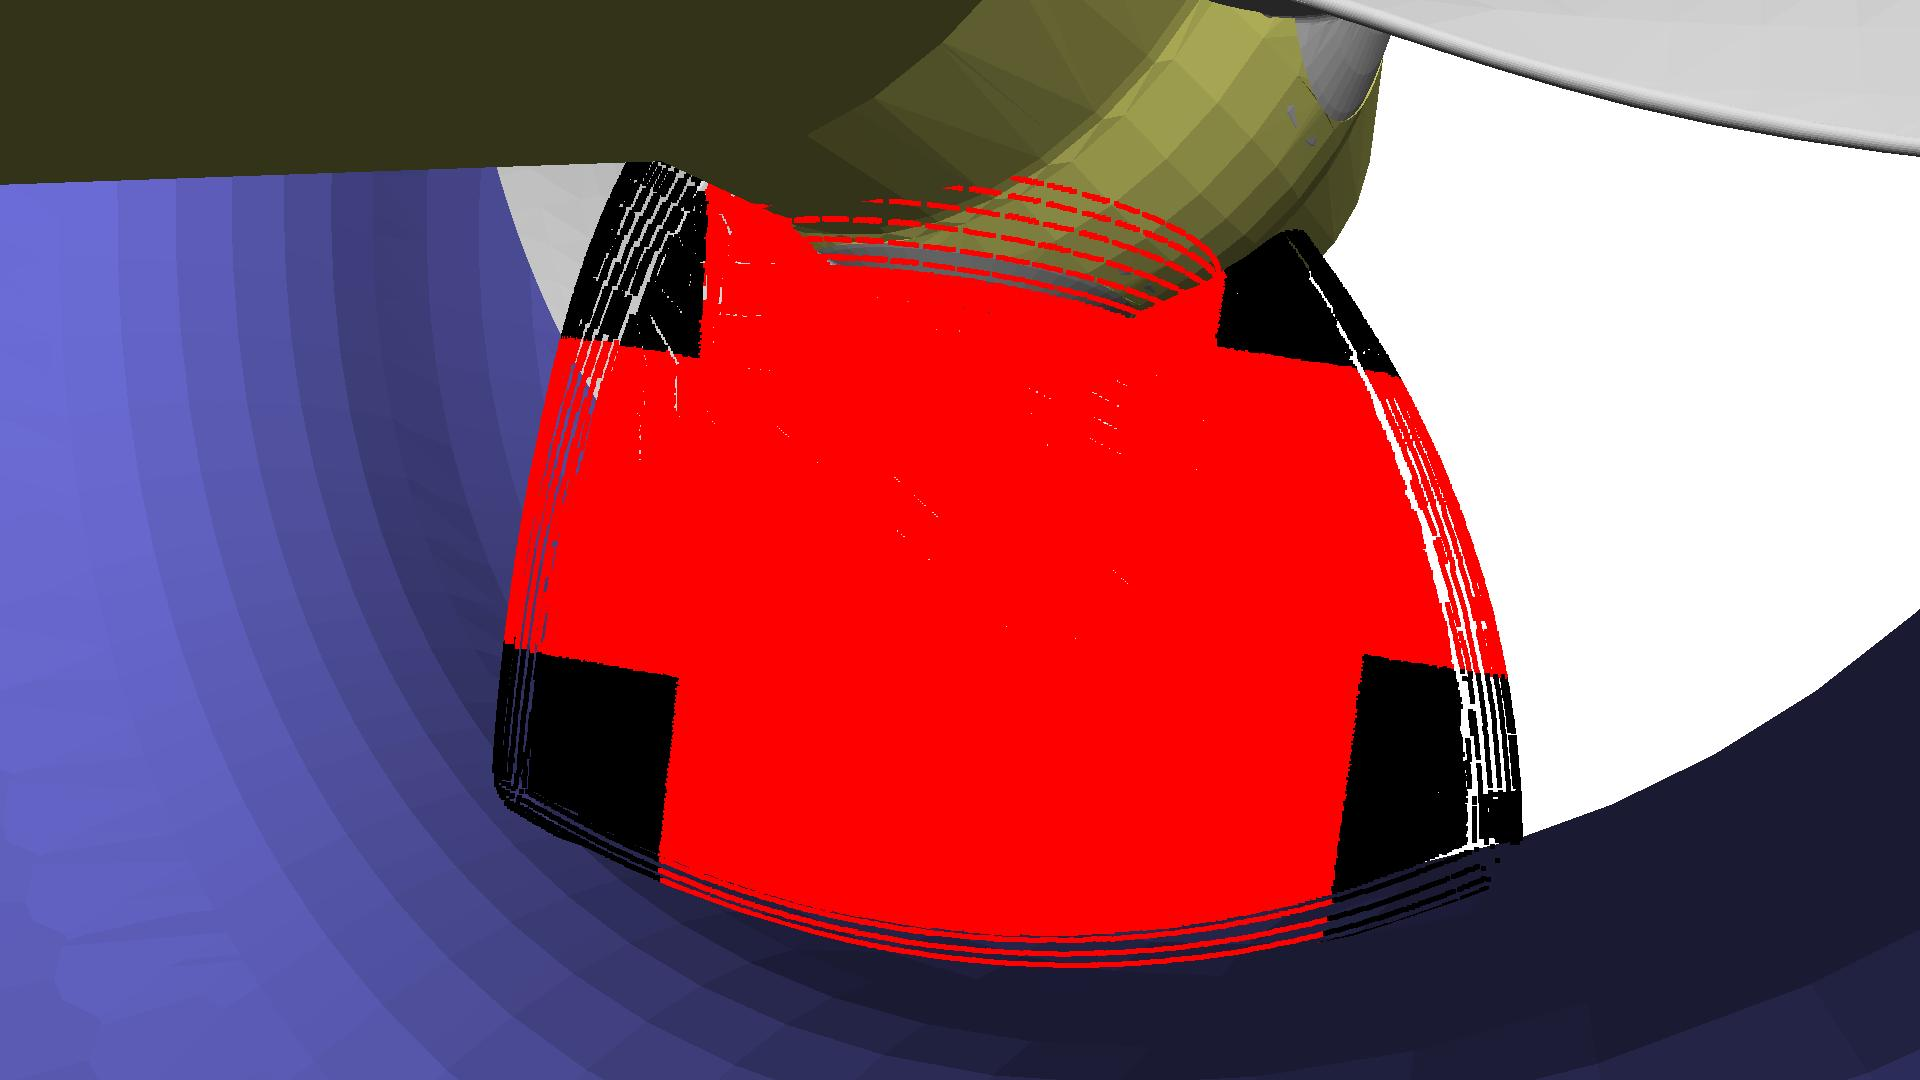
\includegraphics[width=.8\columnwidth]{figs/tocoat.jpg}
	\caption{Extremidades da pá em preto.}
	\label{fig::extremidades}
\end{figure}

\begin{figure}[!ht]
	\centering	
	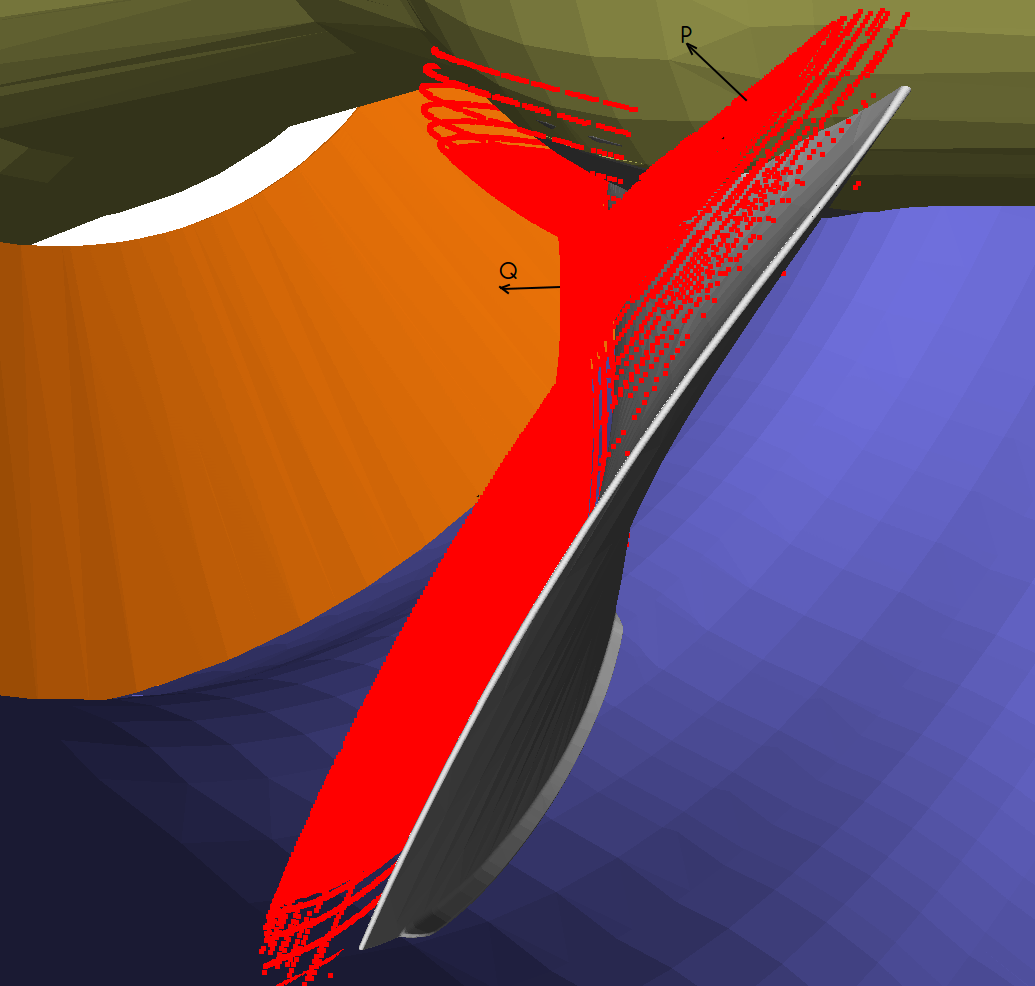
\includegraphics[width=.5\columnwidth]{figs/normal.png}
	\caption{Vetores normais (em preto) de pontos a serem revestidos (em
	vermelho).}
	\label{fig::normal}
\end{figure}

A simulação de teste de revestimento das extremidades considerou as seguintes
variáveis: 

\begin{itemize}
  \item O ângulo das pás da turbina foram fixados em $24^o$, ângulo natural de
  uso.
  \item O rotor da turbina foi girado de $0^o$ a $30^o$ com passo de $3^o$.
  \item A distância entre extremidade da pistola e pá pode variar $235
  \pm 5$ mm.
  \item O ângulo entre a pistola e o plano da pá pode variar $90^o \pm
  30^o$.
  \item A posição em $y$ do robô pode variar $-2970 \pm 250$ mm (posição
  global).
  \item A posição em $x$ do robô pode variar $1500 \pm 250$
\end{itemize}
